\documentclass[11pt,a4paper]{article}

% Preamble: Configuración básica del documento
\usepackage[utf8]{inputenc}
\usepackage[margin=1in]{geometry}
\usepackage{amsmath,amssymb}
\usepackage{xcolor}
\usepackage{listings}
\usepackage{graphicx}
\usepackage{hyperref}

% Configuración de hipervínculos
\hypersetup{
    colorlinks=true,
    linkcolor=teal,
    urlcolor=blue,
    pdftitle={Ruta de Aprendizaje: Dominando LaTeX desde las Bases},
    pdfauthor={Jair Aguilar Peña}
}

% Estilo para fragmentos de código en el documento
\definecolor{codebg}{rgb}{0.96,0.96,0.94}
\definecolor{commentgreen}{rgb}{0,0.5,0}
\definecolor{keypurple}{rgb}{0.5,0,0.5}
\lstdefinestyle{latexstyle}{
    backgroundcolor=\color{codebg},
    commentstyle=\color{commentgreen},
    keywordstyle=\color{keypurple}\bfseries,
    basicstyle=\ttfamily\small,
    breaklines=true,
    showstringspaces=false,
    frame=single,
    rulecolor=\color{gray!40},
    language=[LaTeX]TeX
}

\title{Ruta de Aprendizaje: Dominando \LaTeX\ desde las Bases\\ \large Un plan de estudio para la creación de documentos académicos y profesionales}
\author{Diseñado para: Jair Aguilar Peña}
\date{\today}

\begin{document}

\maketitle

\begin{abstract}
Este documento establece una guía metodológica estructurada para que un estudiante principiante adquiera un dominio completo de \LaTeX. La progresión va desde la redacción de notas cotidianas hasta la composición de artículos de investigación y libros estructurados bajo estándares internacionales, pasando por la creación de gráficos vectoriales, tablas complejas e instrumentación de código.
\end{abstract}

\tableofcontents
\newpage

\section{Metodología de Aprendizaje: "Aprender Haciendo"}
Aprender \LaTeX\ es similar a aprender a programar: la teoría se consolida mediante la práctica directa. Para cada hito en esta ruta, se sugiere crear un archivo de pruebas dentro de tu carpeta de prácticas (\texttt{year\_01/quarter\_01/Practice/}) y compilarlo localmente con \texttt{tectonic} para validar visualmente los resultados.

---

\section{Hito 1: Creación de Documentos Simples (Prácticas, Exámenes y Notas)}
\textbf{Objetivo:} Familiarizarse con la sintaxis de marcado, control de fuentes, alineación de texto y estructuración básica.

\subsection{Conceptos Clave a Dominar}
\begin{itemize}
    \item \textbf{Estructura mínima:} El uso de \texttt{\textbackslash documentclass\{article\}}, el preámbulo y el bloque del cuerpo (\texttt{document}).
    \item \textbf{Jerarquía básica:} Organizar texto usando \texttt{\textbackslash section}, \texttt{\textbackslash subsection} y \texttt{\textbackslash subsubsection}.
    \item \textbf{Alineación y espaciado:} Uso de saltos de línea (\texttt{\textbackslash\textbackslash}), saltos de página (\texttt{\textbackslash newpage}), y el comando \texttt{\textbackslash noindent}.
    \item \textbf{Listas:} Manejo de listas no ordenadas (\texttt{itemize}) y ordenadas (\texttt{enumerate}).
\end{itemize}

\subsection{Código Base de Ejemplo}
\begin{lstlisting}[style=latexstyle, caption={Estructura básica para notas}]
\documentclass[11pt,a4paper]{article}
\usepackage[utf8]{inputenc}
\begin{document}
\section{Mi Primera Nota}
Este es el cuerpo de la nota. Aquí explicamos conceptos clave.
\begin{itemize}
    \item Concepto A.
    \item Concepto B.
\end{itemize}
\end{document}
\end{lstlisting}

\subsection{Proyecto Sugerido}
Diseña una **Hoja de Examen o Práctica** para una materia científica que incluya un encabezado simple (Nombre, Fecha, Instrucciones) y una lista numerada de 5 preguntas conceptuales, combinando texto en negrita y cursiva.

---

\section{Hito 2: Documentos Académicos Estructurados y Publicación}
\textbf{Objetivo:} Aprender a maquetar documentos de múltiples capítulos (tesis, reportes) y artículos científicos siguiendo formatos estandarizados.

\subsection{Conceptos Clave a Dominar}
\begin{itemize}
    \item \textbf{Clases de Documentos Avanzadas:} Usar \texttt{report} (ideal para reportes de investigación y tesis cortas) y \texttt{book} (para libros completos con capítulos, partes y apéndices).
    \item \textbf{Creación de Portadas Estilizadas:} Diseño de una portada personalizada sin números de página usando el entorno \texttt{titlepage} con alineación vertical flexible (\texttt{\textbackslash vfill}).
    \item \textbf{Índices Automáticos:} Inserción del índice general (\texttt{\textbackslash tableofcontents}), de figuras (\texttt{\textbackslash listoffigures}) y de tablas (\texttt{\textbackslash listoftables}).
    \item \textbf{Referencias y Bibliografía:} Uso de \texttt{biblatex} (con \texttt{biber}) para citar fuentes bibliográficas de manera automática usando archivos de datos de citas (\texttt{.bib}).
\end{itemize}

\subsection{Código Base de Ejemplo (Portada Académica)}
\begin{lstlisting}[style=latexstyle, caption={Ejemplo de portada académica personalizada}]
\begin{titlepage}
    \centering
    \vspace*{2cm}
    {\huge\bfseries Universidad de Ciencias de Sistemas\par}
    \vspace{1.5cm}
    {\Large\itshape Proyecto de Investigación Cuantitativa\par}
    \vspace{2cm}
    {\huge\bfseries Análisis de Algoritmos Complejos\par}
    \vfill
    {\Large Autor: Jair Aguilar Peña\par}
    \vfill
    {\large \today\par}
\end{titlepage}
\end{lstlisting}

\subsection{Proyecto Sugerido}
Crea una **estructura de reporte científico de dos capítulos** utilizando la clase \texttt{report}. Diseña una portada atractiva usando el entorno \texttt{titlepage}, genera el índice general automáticamente y añade una sección de referencias al final utilizando citas bibliográficas.

---

\section{Hito 3: Elementos Avanzados (Tablas, Matemáticas, Código y Gráficos)}
\textbf{Objetivo:} Dominar los componentes dinámicos y la notación técnica que hacen a \LaTeX\ el estándar de la industria científica.

\subsection{Conceptos Clave a Dominar}
\begin{itemize}
    \item \textbf{Notación Matemática Compleja:} Matrices con corchetes (\texttt{pmatrix}) o llaves (\texttt{Bmatrix}), sistemas de ecuaciones alineados (\texttt{align}), sumatorias, integrales y letras griegas.
    \item \textbf{Tablas Profesionales:} Uso del paquete \texttt{booktabs} para evitar líneas verticales feas y crear tablas limpias usando solo \texttt{\textbackslash toprule}, \texttt{\textbackslash midrule} y \texttt{\textbackslash bottomrule}.
    \item \textbf{Visualización de Código Fuente:} Configuración del paquete \texttt{listings} para colorear sintaxis, mostrar números de línea y auto-ajustar texto (para lenguajes como Rust, C o Python).
    \item \textbf{Gráficas de Datos:} Uso de \texttt{pgfplots} para graficar funciones matemáticas y conjuntos de datos directamente desde el código sin depender de imágenes externas.
    \item \textbf{Diagramas Vectoriales (TikZ):} Dibujo básico de diagramas de flujo y esquemas utilizando nodos (\texttt{node}) y flechas en \texttt{TikZ}.
\end{itemize}

\subsection{Código Base de Ejemplo (Gráfica Matemática)}
\begin{lstlisting}[style=latexstyle, caption={Graficar una función cuadrática directamente}]
\usepackage{pgfplots}
\pgfplotsset{compat=1.18}
% Dentro del cuerpo:
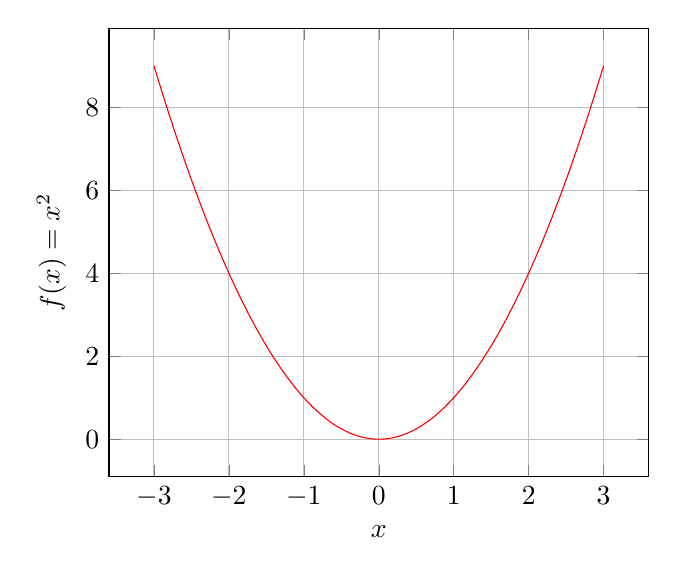
\begin{tikzpicture}
    \begin{axis}[xlabel=$x$, ylabel={$f(x) = x^2$}, grid=major]
        \addplot[color=red, domain=-3:3, samples=100] {x^2};
    \end{axis}
\end{tikzpicture}
\end{lstlisting}

\subsection{Proyecto Sugerido}
Escribe una **nota técnica de matemáticas**. Debe contener:
\begin{enumerate}
    \item Un sistema de ecuaciones lineales resuelto mediante matrices en bloque.
    \item Una tabla que compare el rendimiento de 3 algoritmos utilizando el estilo \texttt{booktabs}.
    \item Un bloque de código de Rust con resaltado de sintaxis.
    \item Una gráfica de una función trigonométrica (por ejemplo, $\sin(x)$) dibujada con \texttt{pgfplots}.
\end{enumerate}

---

\section{Hito 4: Estilización, Formato y Comandos Personalizados}
\textbf{Objetivo:} Adaptar el diseño visual de tus documentos para crear plantillas personales de cuadernos de notas con un toque visual premium.

\subsection{Conceptos Clave a Dominar}
\begin{itemize}
    \item \textbf{Encabezados y Pies de Página:} Uso del paquete \texttt{fancyhdr} para colocar títulos del tema en la parte superior y numeración estilizada en la parte inferior.
    \item \textbf{Diseño de Títulos:} Personalización de fuentes y espaciado de secciones usando \texttt{titlesec}.
    \item \textbf{Comandos Propios (\texttt{\textbackslash newcommand}):} Crear atajos para simplificar tareas repetitivas (por ejemplo, crear un comando rápido para vectores en negrita).
    \item \textbf{Entornos Propios (\texttt{\textbackslash newenvironment}):} Definir bloques personalizados con fondos de color (como cajas de alertas o definiciones matemáticas).
\end{itemize}

\subsection{Código Base de Ejemplo (Comando y Entorno Personalizado)}
\begin{lstlisting}[style=latexstyle, caption={Creación de comandos y entornos personalizados}]
% Comando para escribir un vector en negrita rápido: \vect{x}
\newcommand{\vect}[1]{\mathbf{#1}}

% Entorno para una caja de notas estilizada
\newenvironment{notaimportante}{
    \medskip
    \noindent\color{red!70!black}\textbf{Nota Importante: }
    \itshape
}{
    \medskip
}
\end{lstlisting}

\subsection{Proyecto Sugerido}
Crea tu **plantilla final para Cuaderno de Notas**. Debe incluir encabezados estilizados con el nombre del curso, una macro para resaltar tus dudas conceptuales, y un diseño de sección modificado para que se vea moderno (por ejemplo, con texto en color azul marino o gris oscuro).

---

\section{Recursos de Referencia Recomendados}
Aquí tienes una selección de los mejores recursos de consulta continua clasificados por tipo de medio:

\subsection{Libros de Referencia (Gratuitos en PDF)}
\begin{itemize}
    \item \textbf{Una introducción no muy corta a \LaTeX2e} (Tobias Oetiker): El manual clásico e indispensable. Traducido a decenas de idiomas.\\
    Enlace al PDF oficial en español: \href{https://tobi.oetiker.ch/lshort/lshort-es.pdf}{https://tobi.oetiker.ch/lshort/lshort-es.pdf}
    \item \textbf{Edición de Textos Científicos con \LaTeX} (Alexánder Borbón y Walter Mora): Excelente libro completo con enfoque práctico en matemáticas e ingeniería.\\
    Enlace de descarga del libro completo: \href{https://tecdigital.tec.ac.cr/revistamatematica/Libros/LaTeX/Edicion_de_Textos_Cientificos_con_LaTeX.pdf}{Descargar Libro en PDF}
\end{itemize}

\subsection{Videotutoriales y Cursos Online}
\begin{itemize}
    \item \textbf{Curso Completo de LaTeX desde Cero (YouTube):} Un video tutorial excelente paso a paso impartido en español que te guiará en los primeros pasos y configuraciones.\\
    Enlace de reproducción: \href{https://www.youtube.com/watch?v=F5S9Ld6C7kQ}{Ver Curso en YouTube (Overleaf y LaTeX)}
    \item \textbf{Taller Práctico de LaTeX (YouTube):} Explicación clara y concisa enfocada en la redacción de informes técnicos y ecuaciones.\\
    Enlace del video: \href{https://www.youtube.com/watch?v=kY7_m-L5R2A}{Taller Práctico de LaTeX}
\end{itemize}

\subsection{Sitios Web de Consulta y Comunidades}
\begin{itemize}
    \item \textbf{Learn LaTeX (Interactivo):} Un portal web excelente que te permite ejecutar código de LaTeX directamente en el navegador sin instalar nada.\\
    Página web oficial: \href{https://www.learnlatex.org/es/}{https://www.learnlatex.org/es/}
    \item \textbf{TeX - LaTeX Stack Exchange:} La comunidad de preguntas y respuestas más grande del mundo. Si tienes un error tipográfico o de código, búscalo aquí.\\
    Página web: \href{https://tex.stackexchange.com/}{https://tex.stackexchange.com/}
\end{itemize}

\end{document}
